\chapter{Related Works}
\label{chapter:related}

%\minitoc
\chapterwithfigures{\nameref*{chapter:related}}
\chapterwithtables{\nameref*{chapter:related}}

\ifthenelse{\boolean{skipRelated}}{\endinput}{}

\section{Deep Learning for Computer Vision}

\ac{CNN} have been for a long-time the \textit{defacto} method for \acs{NN} for \ac{CV}
\citep{fukushima1980neocognitron,lecun1999lenet}. In 2012, with larger datasets and better hardware
(\ie \acs{GPU}), \cite{krizhevsky2012alexnet} imposed \ac{DL} models as the best performing
algorithms for images. In the 2010's decade, multiple major improvements were made but the one of
the latest best performing models \citep{tan2019efficientnet} is mainly based on two architectural changes:
residual connections allowing training of very deep networks \citep{he2016resnet} and normalization
of intermediate activations \citep{ioffe2015batchnorm}. Another major factor of recent \ac{CNN}
improvements is better training procedure \citep{wightman2019resnetstrikesback}, which includes
optimizer \citep{kingma2014adam}, learning rate scheduling, strong data augmentations
\citep{muller2021trivialaugment,hingyi2018mixup,zhong2017erasing}, and regularizations
\citep{gal2016dropout,gao2016stochasticdepth}.

More recently, the Transformer architecture \citep{vaswani2017transformer}, originally designed for
machine translation in \ac{NLP}, was applied to images. Using an encoder structure similar to BERT
\citep{devlin2018bert}, ViT \citep{dosovitskiy2020vit} considered patches of pixels as tokens.

\section{Continual Learning}

Usually, when training a \ac{CNN}, we assume the dataset is immutable and \textit{i.i.d.}: no new
image nor new classes will be learned. The knowledge acquired on one dataset A can be
\textit{transferred} to another dataset B with different classes using \textbf{transfer learning}
\citep{razavian2014transferlearning}. However, in that case, the new model, while being efficient on
the dataset B, cannot classify the classes of dataset A.

\textbf{Continual Learning} aims to learn a continually changing dataset without forgetting the
previous knowledge. The distribution of the dataset continually change: at each time-step, \ac{NC},
\ac{NI} from potentially new domains, or even \ac{NIC} are added to the training dataset
\cite{lomonaco2017core50}. We usually assume the test dataset evolves similarly. Continually
learning an ever-growing dataset is doable: a naive but efficient approach consist in training from
scratch a new model on the union of past and new data. However, for multiple reasons like privacy
concerns of medical data or limited storage capacity in embedded device, there is a restriction on
the amount of previous data that can be kept. In the extreme case, where a model only has access to
new data but now old data, training from scratch fails to model previous iterations' distribution.
Worse, even if the old model is kept and finetuned on the new data, it'll suffer from
\textbf{Catastrophic Forgetting} \citep{robins1995catastrophicforgetting}: new data is learned at
the expanse of old data.

\paragraph{Class-Incremental Example} More concretely, a common benchmark in \ac{NC} setting,
commonly called \ac{CIL} is to learn the image classification CIFAR100 dataset
\citep{krizhevskycifar100} in multiple steps, each made of several new classes. \eg a model could
learn at first to classify among 10 classes, then add 10 more classes, \etc. until it has learned
all 100 classes. After each step, the model has to classify among all classes it has learned. The
\autoref{fig:related_forgetting} illustrate such continual training. The \textcolor{orange}{orange}
line displays the accuracy of a model that is re-trained from scratch at each step on all previous
classes data. This model, usually called Joint, is considered as a reasonable upper bound. The
\textcolor{blue}{blue} line on the other hand is a model that is finetuned on new classes but has no
access to previous classes. Evidently, the model's accuracy is much lower than its Joint
counterpart, because it forgets completely old classes by over-predicting new classes.


\paragraph{Single-Head \vs Multi-Heads} are the two main evaluation settings in Continual Learning
\todo{CITE chadhry}. In the former setting, a model has to classify samples among all seen classes,
that could have been learned from any of the seen steps. The latter setting, on the other hand,
knows at test-time from which steps the samples come from. Thus, it only has to classify among the
limited number of classes brought by a step. This setting is closely related to multi-tasks
\todo{CITE}. During this thesis, I focused on the Single-Head setting because it's more realistic
as it is not always possible to know from which step a sample come from in a real-life setting, and
more challenging \citep{lesort2019regulshortcomings}.


\begin{figure}[tb]
    \begin{center}
        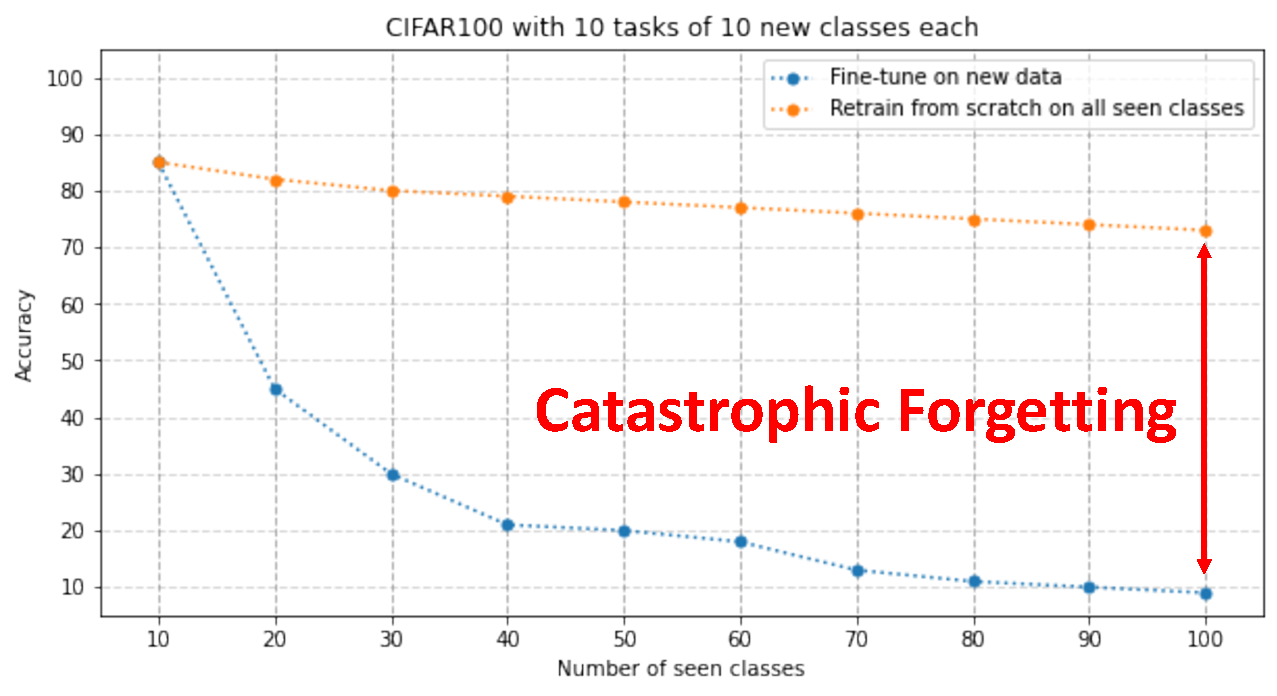
\includegraphics[width=0.8\linewidth]{images/related/catastrophic_forgetting.pdf}
    \end{center}
    \caption{\textbf{Training protocol for incremental learning}. At each training task we learn a
        new set of classes, and the model must retain knowledge about \textit{all} classes. The
        model is allowed a \textit{limited} memory of samples of old classes.}
    \label{fig:related_forgetting}
\end{figure}

\paragraph{Notations} A model trained for image classification has access to a dataset of tuple
$\{\vx, \vy\}$ where $\vx$ is an image, and $\vy$ its class label.

\section{Rehearsal}
\label{sec:related_rehearsal}

Multiple approaches exist to reduce catastrophic forgetting. The most efficient method is
\textbf{rehearsal learning} where old samples will be seen alongside the new samples. The amount of
old samples stored is extremely limited otherwise it would defect the purpose of continual learning.
\autoref{fig:related_protocol} illustrates how rehearsal learning happens in Continual Learning.
During the first step, a model is trained on all available samples. Then, it stores a limited amount
of those in a \textit{memory}. During the second step, the model has access to new samples but also
all samples stored in the memory. In Class-Incremental, an equal amount of samples per class is
stored in memory. Nevertheless, there are two major approaches to determine this amount:
\cite{rebuffi2017icarl} proposed to fully use a memory of size $\mcM$ among all $\mcC$, while
\cite{hou2019ucir} instead kept fixed the amount of samples stored per class to $\nicefrac{\mcM}{|\mcC|}$.

\paragraph{Herding} is the action of choosing which samples per class to store in the rehearsal
memory. The most naive herding method is to sample randomly images. Despite its simplicity, it's
quite competitive with more complex method \citep{castro2018end_to_end_inc_learn}, echoing similar
results in \ac{AL} \citep{gal2017activelearning}. Other herding methods include fetching samples
close to the class mean in the feature space \citep{castro2018end_to_end_inc_learn} or close to an
incremental barycenter \citep{rebuffi2017icarl}.

\paragraph{Sampling} is an important but yet fewly investigated topic in Continual Learning. Most
models mix all memory samples with new samples without any under- or over-sampling.
\cite{castro2018end_to_end_inc_learn} propose to finetune for a few epochs, after training on a new
step, on a balanced set of old and new classes samples. \todo{More on that later}

\paragraph{Efficient Storing} is important for rehearsal learning: a bigger rehearsal memory leads
invariably to less forgetting \citep{douillard2020podnet}. Thus, several works considered how more
samples could be stored given the same memory size: \cite{hayes2020remind} compress intermediate
features of memory samples with a lossless compression algorithm.
\cite{iscen2020incrementalfeatureadaptation} also store features but modify them through the
training to handle the inherent internal covariate shift. \cite{douillard2021objectrehearsal}, in
the context of segmentation, store only non-regular patches of zones of interest instead of storing
the whole, large, images.

\paragraph{Pseudo-rehearsal} doesn't need to store samples, but instead generates pseudo-samples for
rehearsal \citep{lesort2019generative}. The generation can be done with auto-encoders from
intermediate features \citep{kemker2018fearnet,ayub2021eec} or use GAN
\citep{shin2017deep_generative_replay}. Those methods unfortunately have several drawbacks: they
struggle to scale to large images, the generator size may be superior to a classic rehearsal memory
size which would defeat the goal of using less storage, and finally the generator may itself suffer
from catastrophic forgetting. \cite{liu2020mnemonics} propose instead a method halfway between
rehearsal and pseudo-rehearsal: they samples randomly real images, and then during continual
training, slightly modify them via bi-level optimization to minimize forgetting.


\begin{figure}[tb]
    \begin{center}
        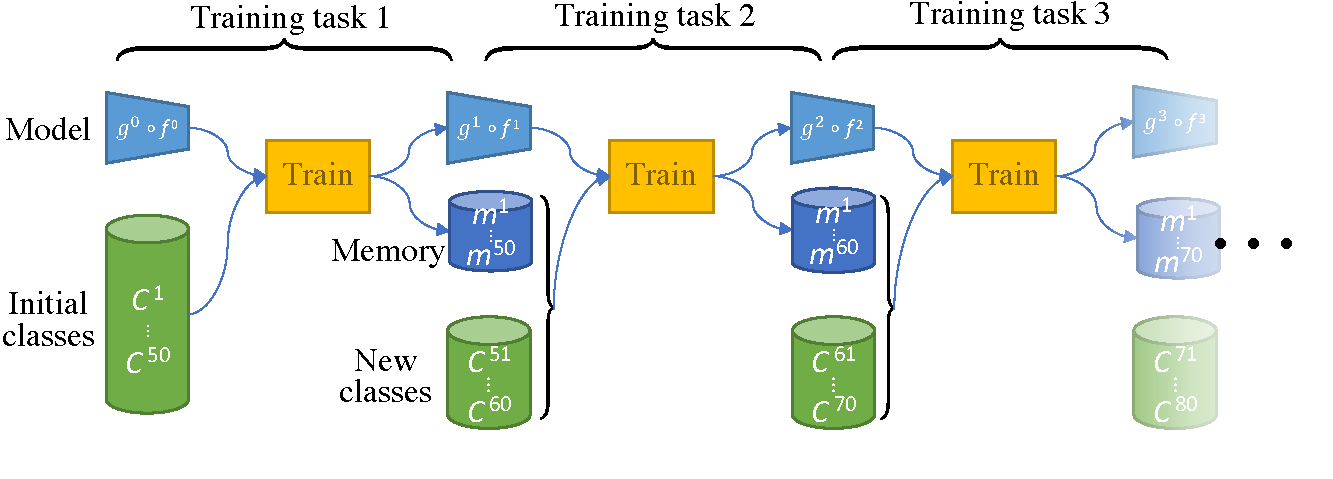
\includegraphics[width=1.0\linewidth]{images/podnet/protocol}
    \end{center}
    \caption{\textbf{Training protocol for incremental learning}. At each training task we learn a
        new set of classes, and the model must retain knowledge about \textit{all} classes. The
        model is allowed a \textit{limited} memory of samples of old classes.}
    \label{fig:related_protocol}
\end{figure}

\autoref{fig:related_protocol}


\section{Regularization-based Approaches}
\label{sec:related_regul}


\begin{figure}[tb]
    \begin{center}
        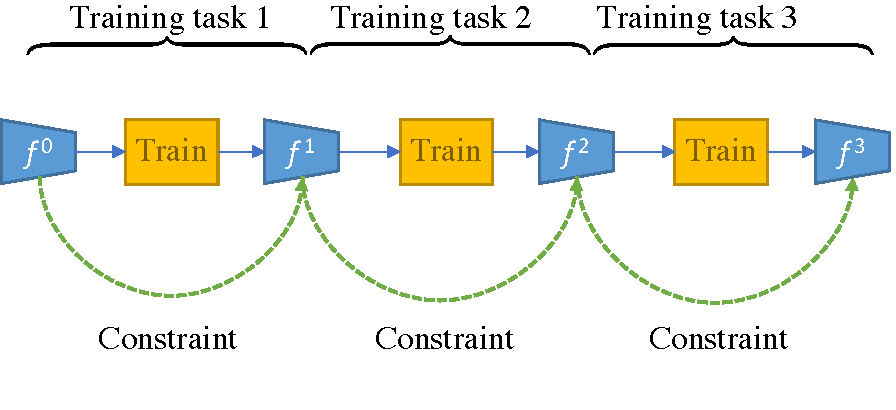
\includegraphics[width=1.0\linewidth]{images/related/continual_regularizations.pdf}
    \end{center}
    \caption{\textbf{Regularizations constraints} forcing the new model to be \textit{similar} to
        the old model to reduce catastrophic forgetting.}
    \label{fig:related_regul}
\end{figure}

A common and efficient way to reduce forgetting, is to minimize the difference in behavior between
the old and new models as illustrated in \autoref{fig:related_regul}. These constraints can be
expressed through various forms as described below.

\subsection{Weight-based}
\label{sec:related_regul_weight}


The most straightforward way to avoid completely forgetting, is that the old and new
models are identical. While the model would be \textit{rigid} (no forgetting), it is also not
\textit{plastic} at all, and thus cannot learn any new tasks. Thus, a line of research proposed to
constrain only a portion of the neurons:
%
\begin{equation}
    \mcL(\theta) = \mcL_\mcT(\theta) + \lambda \sum_i \Omega_i (\theta_i - \theta_i^*)^2\,,
    \label{eq:related_weight_constraint}
\end{equation}
%
where $\mcL_\mcT(\theta)$ is the loss of the current task (\eg the cross-entropy), $\theta_i$ and
$\theta_i^*$ respectively the $i^\text{th}$ neuron of the current and previous model, and $\Omega_i$
a neuron-wise importance factor. The intuition is that important neuron for $\mcT-1$ shouldn't
change, while the others can be adapted to fit the new task $\mcT$.

\cite{kirkpatrick2017ewc}, followed by
\cite{zenke2017synaptic_intelligence} and \cite{chaudhry2018riemannien_walk}
proposed to use the diagonal Fisher information matrix as importance factors.
\cite{aljundi2018MemoryAwareSynapses} instead used the sensitivity of the model when
small perturbations are added to the neurons to measure their importance.

However, it's worth remarking that weight-based constraints are usually limited to the multi-heads
setting where a task identifier is available at test time. \cite{lesort2019regulshortcomings} showed
that in the more realistic single-head setting, they barely reduce forgetting and were significantly
outperformed by rehearsal-based methods.


\subsection{Gradient-Based}
\label{sec:related_regul_gradient}

\cite{lopezpaz2017gem} proposed the GEM model which combines a constraint on the gradients and
rehearsal learning. The algorithm requires that the loss on a given stored sample must not increase
despite the model learning new classes. The authors, given a locality assumption, rewrite this
formulation as enforcing that the gradient of a new sample ($g$) to be in the same \textit{direction} as
the gradient of a stored old sample ($g_i$):
%
\begin{equation}
    \langle g,\, g_i\rangle \ge 0,\, \text{for all} i \in \mcM
\end{equation}
%
With $\mcM$ the rehearsal memory. If the constraint is violated, the new gradient $g$ is projected
to the closest in L2 norm gradient that satisfies the angle constraint by minimizing a quadratic
program. The drawback of this method is the computational cost that can grow prohibitively when the
memory is too large. \cite{chaudhry2019AGEM} proposed Averaged-GEM to speed up GEM: the author don't
constraint the gradient of individual memory samples but only the average of all memory samples.
\cite{aljundi2019gradientselection} also improved GEM's speed by selecting only a subset of the
memory samples that maximize the feasible region.

Differently, but still constraining the gradients: \cite{farajtabar2020ogd}'s OGD forces the gradients of
task $t$ to be orthogonal to gradients of task $t-1$. They use the Gram-Schmidt procedure to
orthogonalize the new gradients, allowing updates for the new task that minimally interfere with the
performance of old tasks. \cite{saha2021gpm}'s GPM does likewise but using instead a k-rank
approximation of the SVD of the representation matrix.


\subsection{Output-based}
\label{sec:related_regul_output}

Finally, the majority of Continual model that are benchmarked on large datasets (\eg ImageNet
\citep{deng2009imagenet}, Pascal VOC \citep{everingham2015pascalvoc}) use a combination of rehearsal
learning (\autoref{sec:related_rehearsal}) and constraints on the model's outputs.

LwF \cite{li2018lwf} and iCaRL applied the \ac{KD} \cite{hinton2015knowledge_distillation} on the
model's probabilities. It usually consists in minimizing the \ac{KL} between the probabilities
of the old and new models:
%
\begin{equation}
    \mcL_\text{KD} = \operatorname{KL}(\operatorname{softmax}(\frac{\tilde{y}^{t-1}}{\tau}) \Vert \operatorname{softmax}(\frac{\tilde{y}^t}{\tau})\,,
\end{equation}
%
where $\tilde{y}^{t-1}$ and $\tilde{y}^{t}$ are respectively the logits of the old and new model,
and $\tau$ a \textit{temperature} to soften the probabilities in order to give more importance to
the \textit{dark knowledge} of \cite{hinton2015knowledge_distillation}. Note that in the context of
Class-Incremental, the new model predicts more classes than the old model, therefore the \ac{KL} is
only applied on the logits common to both the old and the new models. The \ac{KD} is sometimes also
defined as the binary cross-entropy between the sigmoid-activated logits.

Constraining the probabilities is now so ubiquitous that most models include it in their base
losses. On the other hand, a few models considered constraining intermediate outputs. MK2D
\citep{peng2019m2kd} uses the \ac{KD} from both the final classifier and an auxilliary classifier
similarly to the Inception network \citep{szegedy2015inception}. \cite{hou2019ucir} maximizes the
cosine similarity between the embeddings produced by the \ac{GAP}.
\cite{dhar2019learning_without_memorizing_gradcam} minimizes the L1 distance between the attention
maps produced by GradCam \citep{selvaraju2017gradcam}. Drawing inspiration from the model
compression litterature \cite{zagoruyko2016distillation_attention}, \cite{douillard2020podnet}
proposed to constraint instead the statistics of all intermediate features of the \ac{ConvNet}. This
constraint was later expanded to incorporate multiscale information \cite{douillard2020plop}.

\section{Dynamic Strategies}

mask

growed networks

ensembing


\section{Optimization}

working on second order, flat minima

